\documentclass[spanish]{beamer}
\usepackage[ansinew]{inputenc} % Acepta caracteres en castellano
\usepackage[spanish]{babel}    % silabea palabras castellanas
\usepackage{amsmath}
\usepackage{mathtools,cancel} % cancela con una flecha \cancelto{0}{XXXX}
\renewcommand{\CancelColor}{\color{red}} %change cancel color to red
\usepackage{amsfonts}
\usepackage{amssymb}
\usepackage{dsfont}
\usepackage{graphicx}
\usepackage{geometry}
\usetheme{Madrid}
\usecolortheme{beaver}
\usepackage{textpos}
% Logo  en el comienzo 
\addtobeamertemplate{frametitle}{}{%
\begin{textblock*}{100mm}(.85\textwidth,-1cm)
{\includegraphics[height=0.4in, keepaspectratio=true]{/Users/luisnunez/Dropbox/MisDocumentos/UIS/UISImagenInstitucional/UISLOGO.png}}
\end{textblock*}}

\begin{document}

\title{\textbf{Girocomp�s y efecto Coriolis} }
\author[L.A. N��ez]{\textbf{Luis A. N��ez}}  
\institute[UIS]{\textit{Escuela de F�sica, Facultad de Ciencias, } \\
\textit{Universidad Industrial de Santander, Santander, Colombia } \\
{\includegraphics[height=0.4in, keepaspectratio=true]{/Users/luisnunez/Dropbox/MisDocumentos/UIS/UISImagenInstitucional/UISLOGO.png}}
}
\date{\today}
\maketitle


\begin{frame}
\frametitle{Agenda}
  \tableofcontents
\end{frame}


%%%%% Diapo 1
\section{Girocomp�s}
\subsection{Generalidades}
\frame{
\frametitle{Girocomp�s}
\begin{figure}[t]
	\includegraphics[width=1.8in]{Figuras/Girocompas.png}
\end{figure}  
   \begin{itemize}  
  	\item<1-> El girocomp�s, es un instrumento para la navegaci�n inercial, que permite indicar el Norte geogr�fico sin referencia al campo magn�tico.
	\item<2-> Es un disco con momentos principales de inercia $I_{1}^{1}=I_{2}^{2} \neq I_{3}^{3}$, que gira con velocidad angular constante $\omega$, alrededor del eje perpendicular a su plano, que llamamos $x_3$.
	\item<3-> Simult�neamente, el disco puede rotar libremente un �ngulo $\theta$ alrededor de un eje perpendicular a $x_3$. 
    \end{itemize}
}
%
%%%%% Diapo 2
\subsection{Navegaci�n inercial}
\frame{
\frametitle{Navegaci�n inercial}
\begin{figure}[t]
	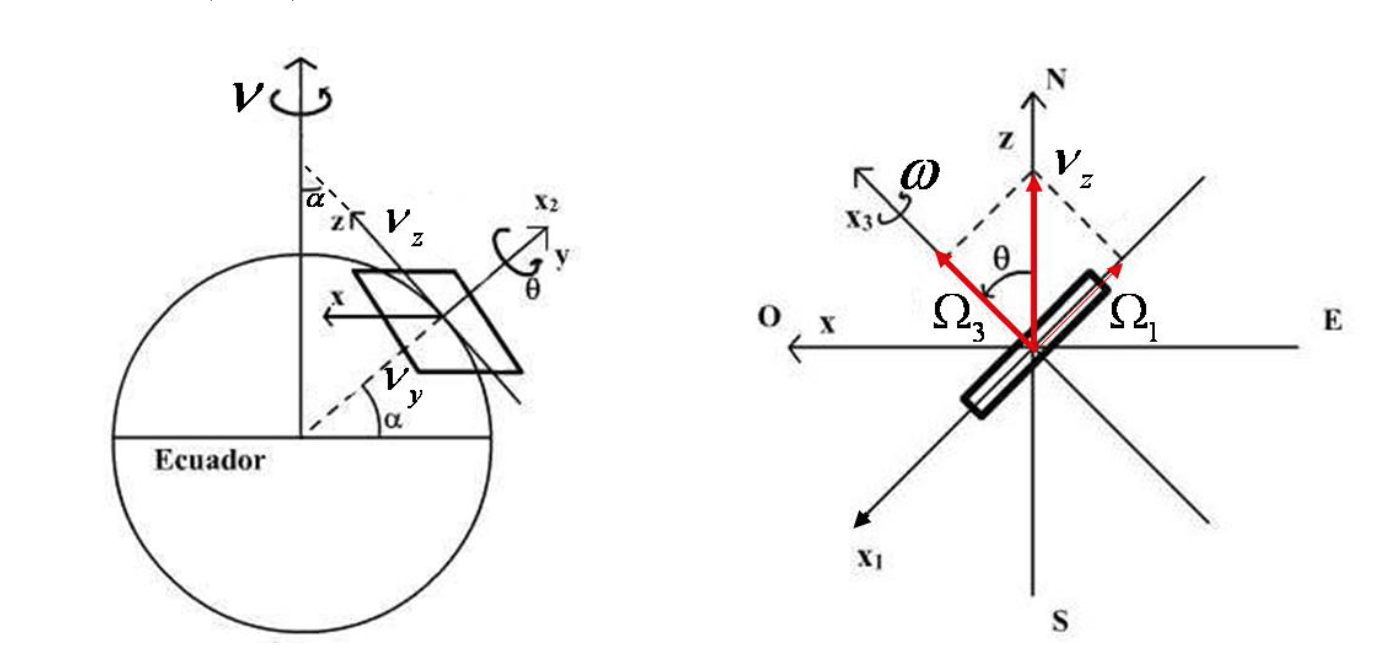
\includegraphics[width=3.5in]{Figuras/GirocompassTierra.png}
\end{figure}
\begin{itemize}  
	\item<1-> Sea $\nu$ la magnitud de la velocidad angular de la Tierra alrededor de su eje NorteSur, con $\omega \gg \nu$, donde $\alpha$ es la latidud.
	\item<2-> El sistema de coordenadas ( $x, y, z$ ) est� fijo en la Tierra y el sistema ( $x_1, x_2, x_3$ ) est� en el CM del disco
	\item<3-> Las componentes de la velocidad angular de la Tierra en ($x, y, z$) son $\nu_x=0, \quad$  $\nu_y=\nu \operatorname{sen} \alpha \quad$ y $\quad \nu_z=\nu \cos \alpha$
\end{itemize}
}
%
%%%%% Diapo 2
\subsection{Las velocidades angulares}
\frame{
\frametitle{Las velocidades angulares}
\begin{itemize}  
	\item<1-> Supongamos que la direcci�n de $\dot{\theta}$ en un instante dado est� sobre el eje $x_2$ (simetr�a del disco permite esta simplificaci�n).
	\item<2-> las componentes de $\boldsymbol{\Omega}$ respecto a $\left(x_1, x_2, x_3\right)$ son: 
	$\left\{
	\begin{aligned}
		\Omega^1 & =-\nu_z \operatorname{sen} \theta=-\nu \cos \alpha \operatorname{sen} \theta \\
		\Omega^2 & =\nu_y+\dot{\theta}=\nu \operatorname{sen} \alpha+\dot{\theta} \\
		\Omega^3 & =\nu_z \cos \theta+\omega=\nu \cos \alpha \cos \theta+\omega
	\end{aligned}
	\right.$
	\item<3-> El instrumento es libre de rotar sobre el eje $y$, no hay componente del torque en direcci�n de $y$, que corresponde instantaneamente al eje $x_2$.
	\item<4-> Entonces, la ecuaci�n de Euler $\tau^2=I_{2}^{2} \dot{\Omega}^2+\Omega_1 \Omega_3\left(I_{1}^{1}-I_{3}^{3}\right)=0$
	\item<5-> Derivando $\Omega^2$ y sustituyendo  (con $I_{1}^{1} = I_{2}^{2}$) tenemos
	$I_{1}^{1} \ddot{\theta}+\left(I_{3}^{3}-I_{1}^{1}\right) \nu \cos \alpha \operatorname{sen} \theta(\nu \cos \alpha \cos \theta+\omega)=0$
	\item<6-> Como $\omega \gg \nu$, entonces $\omega \gg \nu \cos \alpha \cos \theta$, e implica
	$I_{1}^{1} \ddot{\theta}+\left(I_{3}^{3}-I_{1}^{1}\right) \nu \omega \cos \alpha \operatorname{sen} \theta \approx 0 $
	\item<7-> Para peque�as oscilaciones 
	$I_{1}^{1} \ddot{\theta}+\left(I_{3}^{3}-I_{1}^{1}\right) \nu \omega \cos \alpha \; \theta \approx 0 $ 
\end{itemize}
}
%
%%%%% Diapo 2
\subsection{Peque�as Oscilaciones}
\frame{
\frametitle{Peque�as Oscilaciones}
\begin{itemize}  
	\item<1-> Peque�as Oscilaciones $I_{1}^{1} \ddot{\theta}+\left(I_{3}^{3}-I_{1}^{1}\right) \nu \omega \cos \alpha \; \theta \approx 0  \Leftrightarrow  \ddot{\theta}+\omega_c^2 \theta \approx 0$, \\ con lo cual 
	$\omega_c^2=\frac{\left(I_{3}^{3}-I_{1}^{1}\right)}{I_{1}^{1}} \nu \omega \cos \alpha,$
	\item<2-> Es la frecuencia para peque�as oscilaciones del eje $x_3$ del disco alrededor del eje $z$, que apunta hacia el Norte.
	\item<3-> El punto de equilibrio $\theta=0$ de la oscilaci�n del eje $x_3$ se�ala la direcci�n del Norte geogr�fico.
	\item<4-> La frecuencia de oscilaci�n $\omega_c$ permite a su vez calcular la latitud $\alpha$ sin ninguna referencia externa
	\item<4-> $\omega_c=0 \Rightarrow \alpha=\frac{\pi}{2}$ es  Polo Norte.  \\
	$\omega_c=\text { m�xima } \Rightarrow \alpha=0$ es el Ecuador. 
\end{itemize}
}
%
%%%%% Diapo 2
\section{Efecto Coriolis}
\frame{
\frametitle{Efecto Coriolis}
\begin{figure}[t]
	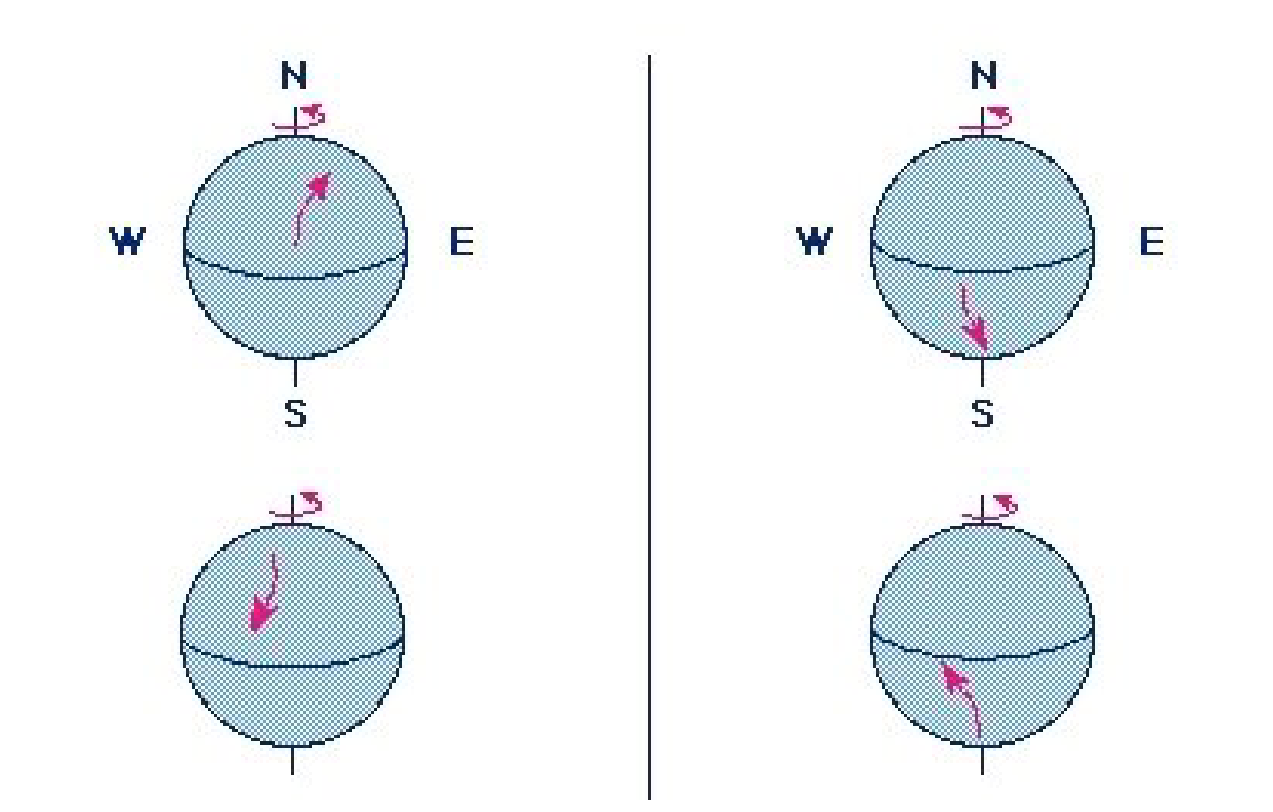
\includegraphics[width=1.8in]{Figuras/Coriolis.png}
\end{figure}
\begin{itemize}  
	\item<1-> Sea (${\bf x}, {\bf y}, {\bf z}$) un sistema inercial (en reposo respecto a las estrellas fijas) y (${\bf x}_1, {\bf x}_2, {\bf x}_3$) un sistema de coordenadas en rotaci�n (la Tierra) con velocidad angular constante $\boldsymbol{\Omega}$ relativa al sistema inercial.
	\item<2-> Una vez mas 
	$\left(\frac{d {\bf r}}{d t}\right)_{(x, y, z)}=\left(\frac{d {\bf r}}{d t}\right)_{\left(x_1, x_2, x_3\right)}+\boldsymbol{\Omega} \times {\bf r} \equiv {\bf v}^{\prime} + \boldsymbol{\Omega} \times {\bf r},$
	\item<3-> Con lo cual $\frac{d {\bf v}}{d t}=\frac{d {\bf v}^{\prime}}{d t}+ \boldsymbol{\Omega} \times {\bf v} \equiv \frac{d {\bf v}^{\prime}}{d t} + \boldsymbol{\Omega} \times {\bf v}^{\prime} +\boldsymbol{\Omega} \times\left({\bf v}^{\prime} + \boldsymbol{\Omega} \times {\bf r}\right)$
	\item<4-> Entonces $\underbrace{m \frac{d \mathbf{v}}{d t}}_{\bf F}=\underbrace{m\frac{d {\bf v}^{\prime}}{d t}}_{\bf F^{\prime}} +\underbrace{2 m \boldsymbol{\Omega} \times {\bf v}^{\prime}}_{-{\bf F}_{Coriolis}}+ \underbrace{ m \boldsymbol{\Omega} \times (\boldsymbol{\Omega} \times \mathbf{r})}_{-{\bf F}_{centrifuga}}$
	\item<5-> Es decir ${\bf F}^{\prime} = {\bf F} +{\bf F}_{Coriolis} +{\bf F}_{centrifuga}$  
\end{itemize}
}


%%%%% Diapo Fin
\section{Recapitulando}
\frame{
  \frametitle{Recapitulando}
En presentaci�n consideramos
  \begin{enumerate}
  	\item<1->
   \end{enumerate}
}
  
\end{document}

%
%%%%% Diapo 2
\section{Secci�n}
\frame{
\frametitle{T�tulo transparencia}
\begin{itemize}  
	\item<1-> 
\end{itemize}
}


	\begin{figure}[t]
		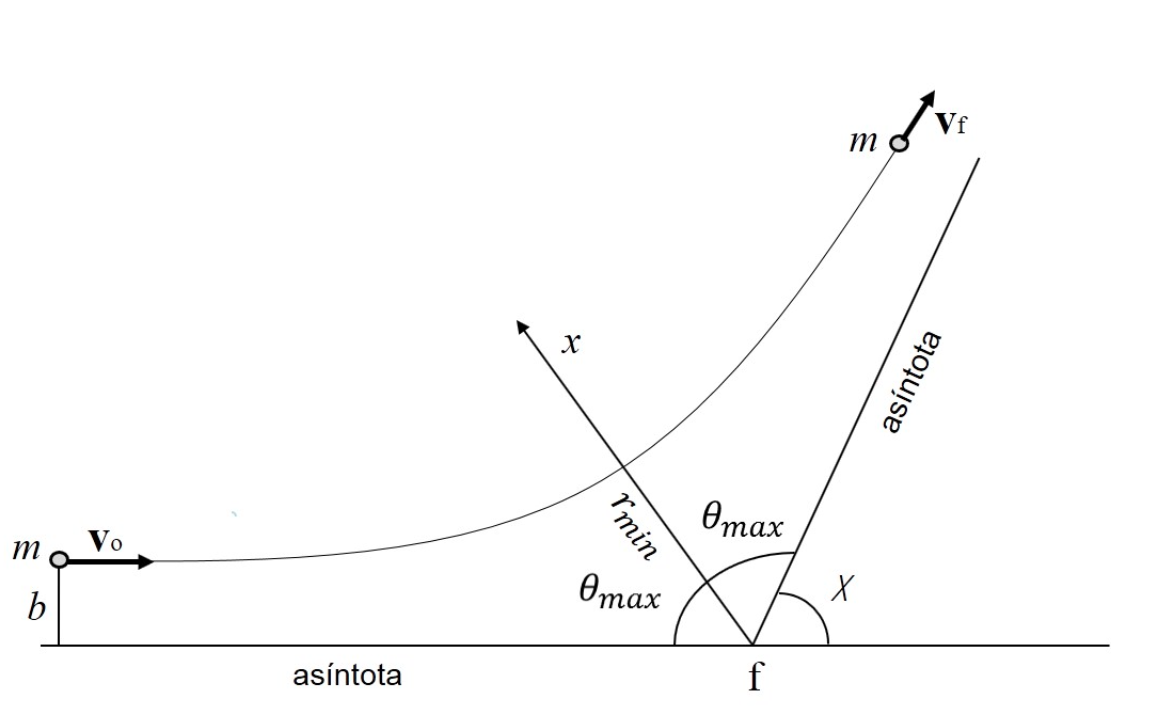
\includegraphics[width=1.8in]{Figuras/Dispersion.png}
   	\end{figure}
	
